\chapter{Eigenvalues and Eigenvectors}
Given a matrix \( A \) of size \( n \times n \) and a scalar \( \lambda \) and a vector \( \mathbf{x} \neq \mathbf{0} \) such that
\[
A\mathbf{x} = \lambda \mathbf{x},
\]
then \( \lambda \) is said to be an eigenvalue of \( A \), and \( \mathbf{x} \) is said to be an eigenvector of \( A \).

To compute \( \lambda \), we can proceed as follows:
\begin{align*}
A\mathbf{x} &= \lambda \mathbf{x} \\
A\mathbf{x} - \lambda \mathbf{x} &= \mathbf{0} \\
(A - \lambda I)\mathbf{x} &= \mathbf{0}
\end{align*}

Here we have a homogeneous linear system. From the theory, we know that if the matrix has maximum rank,
then there is only a unique solution which is the trivial solution. But given the definition above, in this
case \( \mathbf{x} \neq \mathbf{0} \), this implies that necessarily the matrix \( A - \lambda I \) must be
singular so the determinant of \( A - \lambda I \) must equals to zero
\[
\det(A - \lambda I) = 0
\]
The determinant \( \det(A - \lambda I) \) is a polynomial in the unknown \( \lambda \),
which is called the characteristic polynomial. The roots of this polynomial will be the
eigenvalues of \( A \).

All the eigenvalues of \( A \) form the spectrum of \( A \), denoted as 
\[
\sigma(A) = \{ \lambda_1, \lambda_2, \ldots, \lambda_n \}.
\]

The pair \( (\lambda, \mathbf{x}) \) is called an eigenpair of \( A \).

If \( \mathbf{x} \) is an eigenvector of \( A \), then by definition
\[
(A - \lambda I)\mathbf{x} = \mathbf{0} \quad \Rightarrow \quad \mathbf{x} \in \underbrace{\mathcal{N}(A - \lambda I)}_{\text{Eigenspace}},
\]

\textbf{Example.} Compute the eigenvalues and eigenvectors of the matrix $A$
\[
A = \begin{pmatrix}
4 & -5 \\
2 & -3
\end{pmatrix}.
\]
1. Write \((A - \lambda I)\) and set the determinant to zero to find the characteristic polynomial.

$$ A - \lambda I = \begin{pmatrix}
4 & -5 \\
2 & -3
\end{pmatrix} - \begin{pmatrix}
\lambda & 0 \\
0 & \lambda
\end{pmatrix} = \begin{pmatrix}
4 - \lambda & -5 \\
2 & -3 - \lambda
\end{pmatrix} $$


\begin{align*}
    \det \begin{pmatrix}
        4 - \lambda & -5 \\
        2 & -3 - \lambda
        \end{pmatrix} &= (4-\lambda)(-3-\lambda) - (-10) \\
        &= -12 - 4\lambda + 3\lambda + \lambda^2 + 10 \\
        &= \lambda^2 - \lambda - 2 = 0
\end{align*}
\[
\lambda = \frac{-(-1) \pm \sqrt{(-1)^2 - 4(1)(-2)}}{2(1)} = \frac{1 \pm \sqrt{9}}{2} = \frac{1 \pm 3}{2}
\]
Thus, we get \(\lambda_1 = 2\) and \(\lambda_2 = -1\).

2. Computation of eigenvectors: \newline

For \((A - \lambda I)X = 0\), solve the system:
\[ (A - \lambda_1 I)X = \left[\begin{pmatrix} 4 & -5 \\ 2 & -3 \end{pmatrix} - \begin{pmatrix} 2 & 0 \\ 0 & 2 \end{pmatrix}\right] X = \mathbf{0} \]
This simplifies to:
\[
\begin{pmatrix}
2 & -5 \\
2 & -5
\end{pmatrix} \begin{pmatrix}
x_1 \\
x_2
\end{pmatrix} = \mathbf{0}
\]
For \(\lambda_1 = 2\), we get \(2x_1 - 5x_2 = 0\). Solving for \(x_1\), we have \(x_1 = \frac{5}{2} x_2\).

The general solution is:
\[
\begin{pmatrix}
x_1 \\
x_2
\end{pmatrix} = x_2 \begin{pmatrix}
5/2 \\
1
\end{pmatrix}
\]
Thus, \(X_1 = \begin{pmatrix}
5/2 \\
1
\end{pmatrix}\) is an eigenvector.

Repeat the process for \(\lambda_2\) to find the second eigenvector.
\subsection{Complex Eigenvalues for Real Matrices}

\begin{itemize}
    \item A matrix \( A \) with real entries can have complex eigenvalues.
    \item If a matrix \( A \) with real entries has an eigenvalue \( \lambda \in \mathbb{C}\),
    then also the conjugate \(\bar{\lambda}\) is an eigenvalue of \( A \).
\end{itemize}
If \( \lambda \in \mathbb{C} \) is an eigenvalue then $ A\mathbf{x} = \lambda\mathbf{x} \quad \mathbf{x} \neq 0$. If we consider its complex conjugate, we get:
\begin{align*}
    \overline{A\mathbf{x}} = \overline{A}\overline{\mathbf{x}} &= A\overline{\mathbf{x}} \\
    A\mathbf{x} &= \lambda\mathbf{x} \Rightarrow\overline{(A\mathbf{x})} = \overline{\lambda\mathbf{x}} \\
    &\Rightarrow A\bar{\mathbf{x}} = \bar{\lambda}\bar{\mathbf{x}} \quad \Rightarrow \quad \bar{\lambda} \text{ is also an eigenvalue of } A
\end{align*}

\subsection{Eigenvalues of \( 2 \times 2 \) Matrices}
For \( 2 \times 2 \) matrices the following holds:
\begin{align*}
    A = \begin{pmatrix} a & b \\ c & d \end{pmatrix}
    \quad
    \begin{aligned}
        trace(A) &= a + d \\
        det(A) &= ad - bc\
    \end{aligned}
\end{align*}
To compute \( \lambda \) if we assume the characteristic equation:

\begin{align*}
    det(A - \lambda I) &= det \begin{pmatrix} a - \lambda & b \\ c & d - \lambda \end{pmatrix} \\
    &= (a - \lambda)(d - \lambda) - bc \\
    &= ad - a\lambda - \lambda d + \lambda^2 - bc \\
    &= \lambda^2 - \lambda(\underbrace{a + d}_{trace(A)}) + \underbrace{ad - bc}_{det(A)} \\
\end{align*}

$$ \lambda = \frac{trace(A) \pm \sqrt{trace(A)^2 - 4 \cdot det(A)}}{2} $$
In general, we have
\begin{align*}
    \sum_{i=1}^{n} \lambda_i &= trace(A) \\
    \prod_{i=1}^{n} \lambda_i &= det(A)
\end{align*}

\textbf{Theorem:}
If a matrix \( A \) is singular then it has at least one null eigenvalue.

\textbf{Proof:}
If the matrix \( A \) is singular its determinant is zero:
\[
    det(A) = 0 \Rightarrow \prod_{i=1}^{n} \lambda_i = 0 \Rightarrow \exists i: \lambda_i = 0.
\]

Given a matrix \( A \) of size \( m \times m \) which is diagonal:
\[
A = \begin{pmatrix}
d_{11} & 0 & \cdots & 0 \\
0 & d_{22} & \cdots & 0 \\
\vdots & \vdots & \ddots & \vdots \\
0 & 0 & \cdots & d_{mm}
\end{pmatrix}
\]

What are its eigenvalues?

\begin{enumerate}
    \item We construct \( (A - \lambda I) \)
    \item Compute \( \text{det}(A - \lambda I) \):
    \[
        det \begin{pmatrix}
        d_{11} - \lambda & 0 & \cdots & 0 \\
        0 & d_{22} - \lambda & \cdots & 0 \\
        \vdots & \vdots & \ddots & \vdots \\
        0 & 0 & \cdots & d_{mm} - \lambda
        \end{pmatrix} = (d_{11} - \lambda)(d_{22} - \lambda) \cdots (d_{mm} - \lambda) = 0
    \]
    \[
        d_{11} = \lambda_1, \quad d_{22} = \lambda_2, \quad \ldots, \quad d_{mm} = \lambda_m
    \]
\end{enumerate}
Also for Triangular matrices: The eigenvalues of the elements on the main diagonal.

\begin{itemize}
\item The eigenvalues of \( A \) are the same as the eigenvalues of \( A^T \).
\item The eigenvalues of \( A^k \) are equal to the k-th power of the eigenvalues of \( A \).
    \begin{align*}
        A\mathbf{x} &= \lambda \mathbf{x} \\
        A^2\mathbf{x} &= A(A\mathbf{x}) = A(\lambda \mathbf{x}) = \lambda (A\mathbf{x}) = \lambda^2 \mathbf{x} \\
        A^3\mathbf{x} &= A(A^2\mathbf{x}) = A(\lambda^2 \mathbf{x}) = \lambda^2 (A\mathbf{x}) = \lambda^3 \mathbf{x} \\
        \vdots \\
        A^k\mathbf{x} &= \lambda^k \mathbf{x}
    \end{align*}
\item If a given matrix $A$ is not singular and $\lambda$ is an eigenvalue of $A$, then $\lambda^{-1}$ is an eigenvalue of the inverse matrix.
    \begin{align*}
        A\mathbf{x} &= \lambda \mathbf{x} , \quad A \text{ is not singular} \\
        A^{-1}A\mathbf{x} &= A^{-1} \lambda \mathbf{x} \\
        I\mathbf{x} &= \lambda A^{-1} \mathbf{x} \\
        \frac{1}{\lambda} \mathbf{x} &= A^{-1} \mathbf{x}
    \end{align*}
\item For a matrix \( A \) of size \( m \times m \), the number
    $\rho(A) := \max\{|\lambda_1|, |\lambda_2|, \ldots, |\lambda_m|\}$
    is called \textbf{spectral radius} of the matrix $A$.
    We can prove that $\rho(A) \leq ||A||$. \newline
    Let be $\lambda$ an eigenvalue of $A$ and $\mathbf{x}$ the corresponding eigenvector.
    \begin{align*}
        \left\{
        \begin{aligned}
            A\mathbf{x} &= \lambda \mathbf{x} \\
            ||A\mathbf{x}|| &= ||\lambda \mathbf{x}|| = |\lambda| ||\mathbf{x}||\\
            ||A\mathbf{x}|| &\leq ||A|| \, ||\mathbf{x}||
        \end{aligned}
        \right.
        \quad
        \Rightarrow \quad
        ||A\mathbf{x}|| = |\lambda| ||\mathbf{x}|| \leq ||A|| \, ||\mathbf{x}||
    \end{align*}
    This is a generic $\lambda$, so this inequality holds for every eigenvalue of $A$
    therefore it holds for the maximum among the $|\lambda_i|$.
\end{itemize}

\section{Similarity}

Given a matrix \( A \) of size  $m \times m$, it would be useful to transform it into
another matrix of some structure (triangular or diagonal) with the same spectrum.
In particular, we would like to construct what is called a similar matrix.


\textbf{Def.} Given matrices \( A, B \in \mathbb{R}^{m \times m} \), they are said to be \textit{similar} if there exists a non-singular matrix \( S \) such that
\[
S^{-1}AS = B.
\]
This is called a \textbf{similarity transformation}.


\textbf{Proof:} We see that \( B \) has the same spectrum as \( A \). 
Let's say \( \lambda \) be an eigenvalue of \( A \) with \( Ax = \lambda x \) and \( x \neq 0 \). Then,
\begin{align*}
    S^{-1}Ax &= \lambda S^{-1}x \\
    S^{-1}AIx &= \lambda S^{-1}x \\
    S^{-1}A(SS^{-1})x &= \lambda S^{-1}x \\
    (S^{-1}AS)(S^{-1}x) & = \lambda (S^{-1}x) \\
    B(S^{-1}x) & = \lambda (S^{-1}x)
\end{align*}
Setting \( y := S^{-1}x \), we get $By = \lambda y$, which shows \( \lambda \) is an eigenvalue of \( B \) as well.


\textbf{Proposition:} If \( A \in \mathbb{R}^{m \times m} \) has \( m \) linearly independent eigenvectors, then the matrix \( S \) composed of these eigenvectors as columns is such that
\[
S^{-1}AS = \Lambda = \begin{pmatrix}
    \lambda_1 &  & 0 \\
     & \ddots &  \\
    0 &  & \lambda_n
    \end{pmatrix}
\]
where \( \Lambda \) is a diagonal matrix with the eigenvalues of \( A \) on the diagonal.

\textbf{Proof:} Let \( S = \begin{pmatrix} x_1 & x_2 & \dots & x_m \end{pmatrix} \), where \( x_i \) are eigenvectors of \( A \) corresponding to eigenvalues \( \lambda_i \). Then
\[
AS = A\begin{pmatrix} x_1 & x_2 & \dots & x_m \end{pmatrix}
= \begin{pmatrix} Ax_1 &  Ax_2 & \dots &  Ax_m \end{pmatrix}
= \begin{pmatrix} \lambda_1 x_1 & \lambda_2 x_2 & \dots & \lambda_m x_m \end{pmatrix}
= S \Lambda
\]
Thus,
\[
S^{-1}AS = \Lambda.
\]
\textbf{Observation:}
\begin{itemize}
    \item The matrix \( S \) is not unique since we could consider multiples of any eigenvector.
    \item If a matrix \( A \) $n \times n$ has \( n \) distinct eigenvalues, then it has \( n \) linearly independent eigenvectors.
\end{itemize}

\section{Algebraic and Geometric Multiplicity}
\subsection{Algebraic multiplicity}
The \textit{algebraic multiplicity} of a given eigenvalue is the number of times that eigenvalue is a root of the associated characteristic polynomial.

Consider, for example, the polynomial $p(\lambda) = (\lambda - 1)^2$. To compute the roots of $p(\lambda)$:
\begin{align*}
p(\lambda) &= 0 \\
(\lambda - 1)^2 &= 0 \\
(\lambda - 1)(\lambda - 1) &= 0
\end{align*}
This implies that $\lambda = 1$ with algebraic multiplicity equal to $t$.
\textbf{Example:} 
For the matrix 
\[
A = 
\begin{pmatrix}
3 & 1 & 2 \\
0 & 3 & 4 \\
0 & 0 & 3 
\end{pmatrix}
\quad
\lambda = 3 \text{ with algebraic multiplicity} = 3
\]

\subsection{Geometric multiplicity}
The \textit{geometric multiplicity} of a given eigenvalue is the dimension of the associated eigenspace: $$dim(\mathcal{N}(A - \lambda I))$$
\paragraph{Example:}
For the matrix 
\[
A = 
\begin{pmatrix}
3 & 1 \\
0 & 3 
\end{pmatrix}
\]
$(A - \lambda I) = 
\begin{pmatrix}
0 & 1 \\
0 & 0 
\end{pmatrix}
$ and $\lambda = 3$ with algebraic multiplicity $= 2$.

Thus, 
\[
\mathcal{N}
\left[\begin{pmatrix}
0 & 1 \\
0 & 0 
\end{pmatrix}\right]
= \text{span} 
\left\{ \begin{pmatrix}
0 \\
1 
\end{pmatrix} \right\}
\]
and the geometric multiplicity of $\lambda$ is $1$.

In general, the geometric multiplicity $\leq$ algebraic multiplicity.
When the geometric multiplicity $=$ algebraic multiplicity, then the eigenvalues
are said to be \textit{semi-simple}. When the eigenvalues are all distinct,
they are said to be \textit{simple}. We can show that if a matrix $A$ has 
either distinct or semi-distinct eigenvalues, then it has a set of linearly
independent eigenvectors.

\section{Diagonalizability}

\textbf{Question:} When is a given matrix \( A \) similar to a diagonal matrix?

\textbf{Answer:} If the matrix \( A \) has a complete set of eigenvectors, then it's said to be diagonalizable.

A matrix \( A \) has a complete set of eigenvectors if the eigenvectors are linearly independent.

For example, if the given matrix \( A \) does not have a complete set of eigenvectors, then \( A \) is said to be defective.

We cannot diagonalize defective matrices.

For example, consider the matrix
\[
A = \begin{pmatrix}
3 & 1 \\
0 & 3 
\end{pmatrix}
\]
\( \lambda = 3 \) with algebraic multiplicity \( = 2 \) and \( \ker(A - \lambda I) = \) span \( \left\{ \begin{pmatrix} 1 \\ 0 \end{pmatrix} \right\} \), only one linearly independent eigenvector. Therefore, \( A \) is not diagonalizable.

Diagonalizability is not the hard to achieve in practice and there are several numerical methods that can be used. However, when asking if a given matrix \( A \) could be similar to a diagonal matrix, we ask if it could be similar to a triangular matrix.

\subsection{Schur's Triangularization Theorem}

Every square matrix is unitarily similar to an upper triangular matrix.

This means that there exist a matrix \( Q \) such that 
\[ Q^*AQ = T \]
with \( T \) upper triangular.

Note: \( Q \in \mathbb{C} \) is unitary if \( Q^*Q = I \).

\textbf{Theorem: Real Schur Canonical Form}

Given a matrix \( A \) with real coefficients there exists an orthogonal matrix \( Q \) with real coefficients such that
\[ Q^T AQ = T \]
with \( T \) quasi-upper triangular.

This means that the diagonal elements of \( T \) are either \( 1 \times 1 \) blocks or \( 2 \times 2 \) blocks with complex-conjugate eigenvalues.

\section{Application to Spectral Clustering}

Given a dataset \( X \) of points we would like to cluster them using "meaningful groups". Our aim is to keep similar clustering algorithms based on some "distance" measure, but unfortunately, when the set is not convex for example, those algorithms are prone to fail. Hence we need to resort to a different kind of clustering such as spectral clustering.

This means we need to find a more "global" method of representation.

\subsection{Similarity Graph}

To model the local neighborhood relations between data points in \( X \) as a graph where
\textbf{nodes} are the data points and \textbf{edges} are the connections between the points.
If the \textbf{distance} between node \( i \) and node \( j \) is natural, then we have an 
edge between node \( i \) and node \( j \). The edges are weighted by \textbf{similarity}:
\[ s_{ij} = \exp\left(-\frac{dist(i,j)}{\sigma}\right)^2 \]

where \( dist(i,j) \) is the distance between node \( i \) and node \( j \).

We collect \( s_{ij} \) into a matrix \( S \) which is the adjacency matrix of the constructed graph.
\begin{mdframed}
    Note:
    \begin{itemize}
        \item This matrix \( S \) is symmetric.
        \item If any \( S_{ij} = 0 \) then node \( i \) and node \( j \) are not connected.
    \end{itemize}
\end{mdframed}
    
% Degree matrix D
We define the degree matrix \( D \) as a diagonal matrix such that the diagonal 
entry \( D_{ii} \) is the sum of the weights of the edges attached to vertex \( i \),
that is,
$$ D_{ii} = \sum_{j=1}^{n} s_{ij}. $$

\subsection{Laplacian Matrix}

\begin{itemize}
    \item The Laplacian matrix \( L := D - S \)
    \item The normalized Laplacian is given by $L_{u} = D^{-1} L$
    \item The normalized symmetric Laplacian $ L_s = D^{-1/2} S D^{-1/2}$
\end{itemize}


\subsection{Computing Eigenvectors}

% Computing eigenvectors
To compute the eigenvectors and eigenvalues of the Laplacian matrix. In particular,
the number of eigenvalues equal to zero will tell us how many clusters we should create.
Then, taking exactly the same number of eigenvectors, we have a more representative and
different points. This means that in the new representation, the given data in \( X \)
will be "separeted". We can apply a spectral clustering algorithm based on the new basis vectors.

Please have a look at the code \texttt{SpectralClustExample.m} in the Matlab folder.

\section{Power Method to compute the dominant eigenvalue}
Given a matrix $A \in \mathbb{R}^{n \times n}$, with
$\sigma(A) = \{ \lambda_1, \lambda_2, \ldots, \lambda_n \}$, such that
$|\lambda_1| > |\lambda_2| \geq \ldots \geq |\lambda_n|$.
The power method is a strategy to compute the dominant eigenvalue $\lambda_1$ and its corresponding
eigenvector $\mathbf{x}_1$.
In particular, the power method is an iterative procedure that starts from $u_0$ and creates a sequence of
vectors such tat a generic step: $u_{k} = A u_{k-1}$.
The sequence $u_k$ converges to the eigenvector $\mathbf{x}_1$ corresponding to the dominant eigenvalue $\lambda_1$.
How to choose $u_0$ in order to converge to $\mathbf{x}_1$?

Assuming that the set of eigenvectors $\{X_1, \ldots, X_n\}$ of $A$ is linearly independent allows
$u_0 \in \mathbb{R}^n$ to be written as a linear combination of the eigenvectors of $A$:
\[
u_0 = \sum_{i=1}^{n} \alpha_i X_i, \quad \alpha_i \neq 0
\]
Note. $\{X_1, \ldots, X_n\}$ is a basis of $\mathbb{R}^n$.
Let's try to compute few elements of the generated sequence:
$$
\begin{aligned}
  u_1 &= A u_0 = A \sum_{i=1}^{n} \alpha_i X_i = \sum_{i=1}^{n} \alpha_i A X_i = \sum_{i=1}^{n} \alpha_i \lambda_i X_i \\
  u_2 &= A u_1 = A \sum_{i=1}^{n} \alpha_i \lambda_i X_i = \sum_{i=1}^{n} \alpha_i \lambda_i A X_i = \sum_{i=1}^{n} \alpha_i \lambda_i^2 X_i \\
  \vdots \\
  u_k &= A u_{k-1} = A \sum_{i=1}^{n} \alpha_i \lambda_i^{k-1} X_i = \sum_{i=1}^{n} \alpha_i \lambda_i^k X_i \\
  &= \lambda_1^k \left( \alpha_1 X_1 + \sum_{i=2}^{n} \alpha_i \left( \frac{\lambda_i}{\lambda_1} \right)^k X_i \right)
\end{aligned}
$$

When $k \rightarrow \infty$, the ratios $\lambda_i / \lambda_1$ tend to zero for $i \geq 2$ and
the sequence $u_k$ converges to $\lambda_1^k \alpha_1 X_1$.

$$ \lim_{k \rightarrow \infty} u_k = \lambda_1^k\alpha_1 X_1 $$
This means that $u_k \approx \lambda_1^k \alpha_1 X_1$, $u_k$ converges to a multiple of $X_1$.
To compute and approximation of the dominant we need to consider the following "\textbf{Rayleigh quotient}":
At every iteration $k$, we compute the Rayleigh quotient:
$$ \rho_k = \frac{u_k^T A u_k}{u_k^T u_k} $$
Indeed:
$$
\begin{aligned}
  \rho_k &= \frac{u_k^T A u_k}{u_k^T u_k} = \frac{u_k^T u_{k+1}}{u_k^T u_k} =\frac{(\lambda_1^k \alpha_1 X_1)^T (\lambda_1^{k+1} \alpha_1 X_1)}{(\lambda_1^k \alpha_1 X_1)^T (\lambda_1^k \alpha_1 X_1)} \\
  &= \frac{X_1^T\lambda_1X_1}{X_1^TX_1} = \lambda_1\frac{X_1^T X_1}{X_1^T X_1} = \lambda_1
\end{aligned}
$$

In order to make the computation numerically stable, it is recommended to normalize the sequence $u_k$ at every iteration:
the sequence of generated $u_k$.

\begin{enumerate}
    \item We start from $u_0$ which in practice is chosen as a random vector with norm equal to $1$.
    \item At every iteration $k$, we compute $u_{k + 1} = A u_k$
    \item At every iteration $k$, we normalize $z_{k + 1} = \frac{u_{k + 1}}{\|u_{k+1}\|}$.
    \item At every iteration $k$, we compute the Rayleigh quotient $\rho_k = \frac{z_k^T A z_k}{z_k^T z_k}$.
\end{enumerate}

In order to stop the iterative procedure we need to set a suitable stopping criterion.
Firstly, always set a maximum number of iterations to ensure that the procedure will not run indefinitely.
Secondly, it is also fundamental to control the accuracy of the computed quantities. This is done by considering useful error estimates.
For example:
\begin{itemize}
    \item \(\left\| \lambda_k - \lambda_{k+1} \right\| \) : estimate for the absolute error \(\left\| \lambda_k - \lambda_1 \right\|\)
    \item $\frac{|\lambda_k - \lambda_{k+1}|}{|\lambda_{k+1}|}$: estimate fro the relative error $\frac{|\lambda_k - \lambda_1|}{|\lambda_1|}$
    \item $\frac{|\lambda_k - \lambda_{k+1}|}{atol \cdot |\lambda_{k+1}|\cdot rtol}$: estimate for the `mixed' error where $atol$ and $rtol$ are the absolute and relative tolerance respectively.
\end{itemize}

\section{Application of the Power Method to PageRank}
This algorithm is a way to denote the importance of web pages. The importance is measured by counting how many other pages link to the considered web page and also how much important is any of those pages.

If a given page $P_j$ has $l_j$ links and if any of those links comes to a page $P_i$, then we say: ``Page $P_j$ transfers $\frac{1}{l_j}$ of its importance to page $P_i$.''

\paragraph{Rank of a web page}
The rank of a given web page $P_i$ is the sum of all the contributions measured by the pages that link to $P_i$. For pages $P_j \in B_i$, we have:
\begin{equation} \label{eq:rank}
    I(P_i) := \sum_{P_j \in B_i} \frac{I(P_j)}{l_j}
\end{equation}
$B_i$: set of web pages that link to $P_i$.

We construct the so-called \textbf{hyperlink matrix} $H$:
\[
H_{ij} = 
\begin{cases} 
\frac{1}{B_j} & \text{if } P_j \in B_i, \\
0 & \text{otherwise}.
\end{cases}
\]

\textbf{Example}
% TODO: fix layout
\begin{minipage}{0.5\textwidth}
\begin{tikzpicture}[>={Latex[length=3mm]}, node distance=2.5cm, main/.style = {circle, draw}]
    % Nodes
    \node[main] (P1) {1};
    \node[main] (P3) [right of=P1] {3};
    \node[main] (P2) [below of=P1] {2};
    \node[main] (P4) [below of=P3] {4};

    % Edges
    \draw[->] (P1) to[bend right] node[left] {$\frac{1}{2}$} (P2);
    \draw[->] (P1) to[bend left] node[above] {$\frac{1}{2}$} (P3);
    \draw[->] (P3) to[bend right] node[left] {1} (P2);
    \draw[->] (P2) to[bend right] node[below] {1} (P4);
    \draw[->] (P4) to[bend right] node[right] {1} (P2);
\end{tikzpicture}
\end{minipage}
\begin{minipage}{0.5\textwidth}
\[
H = 
    \begin{pmatrix}
    0 & 0 & 0 & 0 \\
    \frac{1}{2} & 0 & 1 & 1 \\
    \frac{1}{2} & 0 & 0 & 0 \\
    0 & 1 & 0 & 0
    \end{pmatrix}
\]
\end{minipage}

$H$ is a \textbf{stochastic matrix}:
\begin{itemize}
\item All the elements are non-negative.
\item The sum of the elements per column is 1.
\end{itemize}

Let us denote with $I$ the vector having as entries the importance of every web page.
\[
I = 
\begin{pmatrix}
I(P_1) \\
I(P_2) \\
\vdots \\
I(P_n)
\end{pmatrix}
\]

Equation (\ref{eq:rank}) can be written in matrix form as: $I = HI$.

This means that $I$ is the eigenvector of $H$ corresponding to the eigenvalue $\lambda = 1$.

There are some issues:

\textbf{Example}
\begin{center}
    \begin{tikzpicture}[>={Latex[length=3mm]}, node distance=2.5cm, main/.style = {circle, draw}]
        % Nodes
        \node[main] (P1) {1};
        \node[main] (P2) [right of=P1] {2};
        % Edges
        \draw[->] (P1) -- (P2);
    \end{tikzpicture}
\end{center}

\[
H = 
\begin{pmatrix}
0 & 0 \\
1 & 0
\end{pmatrix}
\]

This situation is called ``dangling nodes'' situation. In this case, by applying $H$ several
times, the resulting eigenvector will tend to be the zero vector.
This is not allowed by the definition of eigenvector but also it is not a possibility realistic
in our physical universe: The importance of the web would be exhausted.
We need to modify the matrix $H$ if it does not handle the dangling nodes.
So a matrix $S$ is constructed as the matrix of $H$ but where there are columns consisting of
just zeros we are going to write the number $\frac{1}{n}$ ($n$: total number of web pages).

\textbf{Example}

\[
H = 
\begin{pmatrix}
0 & 0 \\
1 & 0
\end{pmatrix}
\quad \rightarrow \quad
S = 
\begin{pmatrix}
0 & \frac{1}{2} \\
1 & \frac{1}{2}
\end{pmatrix}
\]

$S$ is still a stochastic matrix.
We also want to ensure that $|\lambda_1| > |\lambda_2| > \ldots > |\lambda_n|$.
In particular in this case, we want to ensure that $\lambda_1 = 1$ then we need to be sure that $|\lambda_2| < 1$.
Hence $S$ should also be:
\begin{itemize}
\item Irreducible: The graph associated to $S$ is strongly connected.
\item Primitive: There exists an integer $k$ such that all the entries of $S^k$ are positive.
\end{itemize}

The final considered matrix is the so called Google matrix $G$:
$$G = \alpha S + \frac{(1 - \alpha)}{n} \mathbf{1}$$
\begin{itemize}
    \item $0 \leq \alpha \leq 1$ is a parameter that can be tuned, optimal value for $\alpha$ is generally $0.85$
    \item $\mathbf{1}$ is a matrix of only ones.
\end{itemize}

Please have a look at the notebook \texttt{Power Method and Google Page Rank.ipynb}.

\section{Jordan Canonical Form}
The Jordan canonical form (or Jordan normal form) of a matrix is a block diagonal matrix that arises from the structure theorem for finitely generated modules over a principal ideal domain.

Given $A$, $n \times n$ matrix, there exists a non-singular matrix $S$ such that with $J$ called Jordan canonical form.
This matric $J$ is a block diagonal matrix with blocks called Jordan blocks.
$$ J = diag(J(\lambda_1), J(\lambda_2), \ldots, J(\lambda_n)) \quad \text{where} J(\lambda_i) \text{ is a Jordan Segment} $$
\subsubsection{Jordan Segment}
How many blocks inside each segment?
$$ J(\lambda_i) = \begin{pmatrix}
J_1(\lambda_i) & & O \\
& \ddots & \\
O & & J_{T_i}(\lambda_i)
\end{pmatrix}
$$
The number of blocks is equal to the geometric multiplicity ($T_i$) of the eigenvalue $\lambda_i$.

\subsubsection{Jordan Block}
A Jordan block corresponding to an eigenvalue $\lambda$ is a square matrix of the form:
\begin{equation}
J_j(\lambda_i) = 
\begin{pmatrix}
    \lambda_i & 1 & & O \\
    & \ddots & \ddots & \\
    & & \ddots & 1 \\
    & & & \lambda_i
    \end{pmatrix}
\end{equation}

\subsection{Properties}
The Jordan canonical form is unique up to the order of the Jordan blocks.
It provides valuable insights into the structure of a linear transformation,
including the geometric and algebraic multiplicities of eigenvalues.

\begin{itemize}
    \item $\sigma(A)$ is the set of eigenvalues of $A$ or equivalently
    the set of roots of the characteristic polynomial of $A$.
    or the diagonal elements of the Jordan canonical form of $A$.
    \item The algebraic multiplicity of an eigenvalue $\lambda_i$ is the number of times it appears each Jordan segment.    
\end{itemize}

\subsection{Example}
\begin{center}
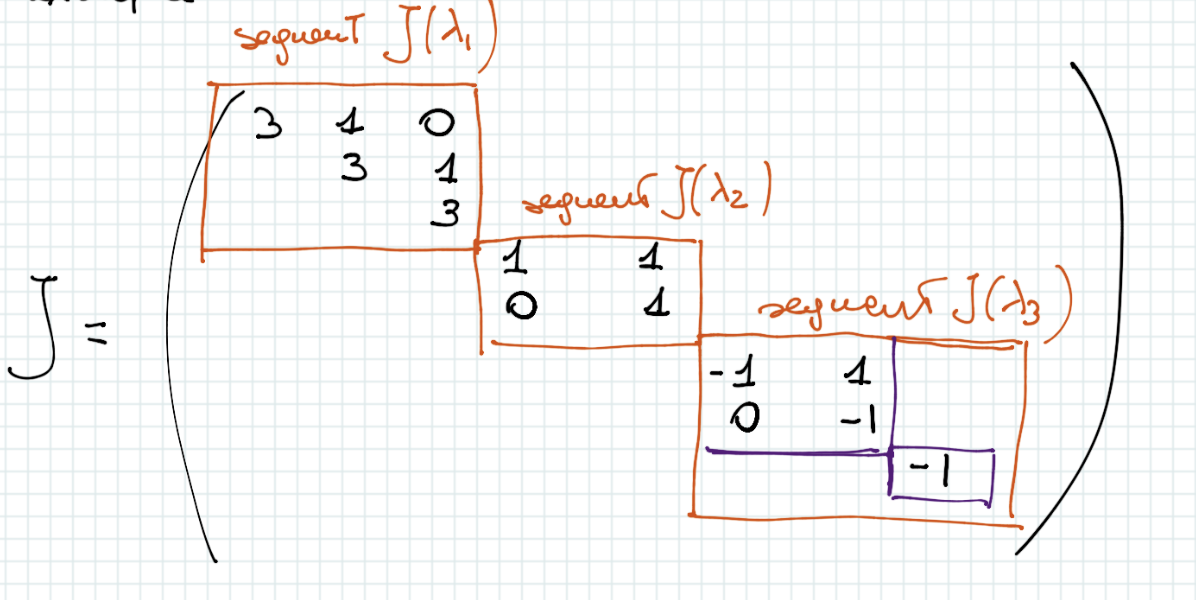
\includegraphics[width=\textwidth,height=\textheight,keepaspectratio]{images/jordan.png}
\end{center}

$\sigma(A)$ is the diagonal elements of $J$: $\sigma(A) = \{\lambda_1 = 3, \lambda_2 = 1, \lambda_3 = -1\}$
The algebraic multiplicity of an eigenvalue $\lambda_i$ is the number of times it appears each Jordan segment.
Hence we have:
\begin{align*}
\text{alg. mult.}(\lambda_1) &= 3 & \text{geom. mult.}(\lambda_1) &= 1 \\
\text{alg. mult.}(\lambda_2) &= 2 & \text{geom. mult.}(\lambda_2) &= 1 \\
\text{alg. mult.}(\lambda_3) &= 3 & \text{geom. mult.}(\lambda_3) &= 2
\end{align*}

Not all matrices are similar to a diagonal matrix. In this case they are said to be defective.
In particular among defective matrices there is the class of nilpotent matrices.
\section{Nilpotent Matrices}
Given a matrix \(N\), \(m \times m\), it is said to be \textbf{nilpotent} whenever \(N^k = 0\) for some positive integer \(k\).

\paragraph{Example}
Consider the matrix
\[
N = \begin{pmatrix}
0 & 1 \\
0 & 0
\end{pmatrix}
\]

\[
N^2 = \begin{pmatrix}
0 & 1 \\
0 & 0
\end{pmatrix}
\begin{pmatrix}
0 & 1 \\
0 & 0
\end{pmatrix}
= \begin{pmatrix}
0 & 0 \\
0 & 0
\end{pmatrix}
\]

\subsection{Core-Nilpotent Decomposition}
Let \( A \) be a \( m \times m \) matrix, singular of index \( k \) such that \( \text{rank}(A^k) = r \), then there exists a non-singular matrix \( Q \) such that
\[
Q^{-1} A Q = \begin{pmatrix}
C & 0 \\
0 & N
\end{pmatrix}
\]
with \( C \) a non-singular matrix of size \( r \times r \) and \( N \) a nilpotent matrix of index \( k \).

In matrix theory, this means that the original matrix \( A \) is similar to a "block-diagonal" matrix with a non-singular core \( C \) and a nilpotent matrix \( N \).


\paragraph{Index}
For a given square matrix \( A \), the \textbf{index} is the smallest non-negative integer \( k \) such that
\[
rank(A^k) = rank(A^{k+1})
\]

\paragraph{Observations}
\begin{itemize}
    \item For non-singular matrices, the index \( = 0 \).
    \item For singular matrices, the index \( > 0 \).
    \item For nilpotent matrices, the index is the smallest integer such that \( N^k = 0 \).
\end{itemize}

General techinique to construct a core-nilpotent decomposition for $2 \times 2$ matrices:
\begin{itemize}
    \item Given $A$, $2 \times 2$ matrix, singular we need to determine its index.
    \item Then we compute $rank(A^k) := z$.
    \item We construct the matrix $Q$ in the following way:
    \[
        Q = \left(X | Y\right)
    \]
    with $X$ of size $2 \times r$ and $Y$ of size $2 \times (2 - r)$.
    $X$ will be found by computing a basis for the range of $A^r$.
    $Y$ will be found by computing a basis for the null space of $A^r$.
    The we compute $Q^{-1}$. This is well-known for $2 \times 2$ matrices.
    If Q is $2 \times 2$ matrix, then
    $$ Q = \begin{pmatrix} a & b \\ c & d \end{pmatrix} \quad Q^{-1} = \frac{1}{ad - bc} \begin{pmatrix} d & -b \\ -c & a \end{pmatrix} $$
    \item As final step we compute $Q^{-1} A Q$ and verify that what we did is correct.
\end{itemize}

\paragraph{Example of core-nilpotent decomposition of a $2 \times 2$ matrix}
\[
A = \begin{pmatrix}
1 & 2 \\
2 & 4
\end{pmatrix} \quad rank(A) = 1
\]
We try to compute the index $k$, if $k = 1$ then $rank(A) = rank(A^2)$.
\[
A^2 = \begin{pmatrix}
1 & 2 \\
2 & 4
\end{pmatrix} \begin{pmatrix}
1 & 2 \\
2 & 4
\end{pmatrix} = \begin{pmatrix}
5 & 10 \\
10 & 20
\end{pmatrix}
\]

So, since $rank(A) = 1$ and $rank(A^2) = 1$ then $k = 1$.
Now we compute a basis for $R(A^k) = R(A)$:
\[
    A = \begin{pmatrix}
    1 & 2 \\
    2 & 4
    \end{pmatrix} \quad \rightarrow \quad
    R_A = \begin{pmatrix}
    1 & 2 \\
    0 & 0
    \end{pmatrix} \quad \rightarrow \quad
    R(A) = span{\left\{ \begin{pmatrix} 1 \\ 2 \end{pmatrix} \right\}}
\]
Next we compute a basis for $N(A^k) = N(A)$:
\[ N(A) = span{\left\{ \begin{pmatrix} -2 \\ 1 \end{pmatrix} \right\}} \]
\[ X = \begin{pmatrix} 1 \\ 2 \end{pmatrix} \quad Y = \begin{pmatrix} -2 \\ 1 \end{pmatrix} \]
\[
    Q = \begin{pmatrix} 1 & -2 \\ 2 & 1 \end{pmatrix}
    \quad Q^{-1} = \frac{1}{5} \begin{pmatrix} 1 & 2 \\ -2 & 1 \end{pmatrix}
\]
\newline
\[
    \begin{aligned}
        Q^{-1} A Q
        &=
        \frac{1}{5} \begin{pmatrix} 1 & 2 \\ -2 & 1 \end{pmatrix}
        \begin{pmatrix} 1 & 2 \\ 2 & 4 \end{pmatrix}
        \begin{pmatrix} 1 & -2 \\ 2 & 1 \end{pmatrix} \\
        &=
        \frac{1}{5} \begin{pmatrix} 5 & 10 \\ 0 & 0 \end{pmatrix}
        \begin{pmatrix} 1 & -2 \\ 2 & 1 \end{pmatrix}  \\
        &=
        \frac{1}{5} \begin{pmatrix} 25 & 0 \\ 0 & 0 \end{pmatrix}
        = \begin{pmatrix} 5 & 0 \\ 0 & 0 \end{pmatrix}
    \end{aligned}
\]

Is the final form correct? Yes!

The core-nilpotent decomposition is a similarity transformation, it's useful when we work with large matrices;
it is preferable to work through transformations as they are numerically stable. 
Hence, it is fair to question: 
"When the core-nilpotent decomposition is also an orthogonal transformation?".
The answer is when it coincides with the URV factorization

Given \( A \), \( m \times m \), then
\[
U R V^T = U
\begin{pmatrix}
C & 0 \\
0 & 0
\end{pmatrix}
V^T = A
\]
with \( U \) and \( V \) orthogonal.


The given matrix \( A \) should be squared with the core-unipotent decomposition:
\[
Q^{-1} A Q = \begin{pmatrix}
C & 0 \\
0 & N
\end{pmatrix}
\]

First the $URV$ factorization can be seen as $ R = U^T A V $, then
we can impose:
\[ R = U^{T}AV = U^TA V \]

The only possibility is that \( U = V \). This is possible only when \( R(A) = R(A^T) \) and \( N(A) = N(A^T) \), or when \( R(A) \perp N(A) \).

This happens for a special class of matrices: Range-Perpendicular-to-Nil space matrices, such as RPN matrices.


Where \( A \), \( m \times m \), and \(\text{rank}(A) = r \) then if \( R(A) = R(A^T) \), \( N(A) = N(A^T) \), \( R(A) \perp N(A) \) then
\[ 
A = U \begin{pmatrix}
C_{r \times r} & 0 \\
0 & 0
\end{pmatrix} U^T
\]
with \( U \) orthogonal matrix. Examples of \( RPN \) matrices are the \textbf{normal} matrices for a matrix it is said to be normal if \( A^T A = AA^T \).

% TODO: Have look at:
% \begin{itemize}
%     \item example 7.8.2 page 592 from Mayer book for the Jordan form
%     \item example 5.10.2 page 396 from Mayer book
%     \item discussion starting from page 407 to 408 from Mayer book
%     \item example 5.12.3 page 409 from Mayer book
% \end{itemize}
